\documentclass{acm_proc_article-sp}
\usepackage[utf8]{inputenc}

\renewcommand{\paragraph}[1]{\vskip 6pt\noindent\textbf{#1 }}
\usepackage{hyperref}
\usepackage{graphicx}
\usepackage{url}

\providecommand{\tightlist}{%
  \setlength{\itemsep}{0pt}\setlength{\parskip}{0pt}}

\title{A Visual Investigation of the Kronos Incident}


% Add imagehandling
\usepackage{graphicx}
% Redefine \includegraphics so that, unless explicit options are
% given, the image width will not exceed the width of the page.
% Images get their normal width if they fit onto the page, but
% are scaled down if they would overflow the margins.
\makeatletter
\def\ScaleIfNeeded{%
  \ifdim\Gin@nat@width>\linewidth
    \linewidth
  \else
    \Gin@nat@width
  \fi
}
\makeatother
\let\Oldincludegraphics\includegraphics
{%
 \catcode`\@=11\relax%
 \gdef\includegraphics{\@ifnextchar[{\Oldincludegraphics}{\Oldincludegraphics[width=\ScaleIfNeeded]}}%
}%

\numberofauthors{2}
\author{
\alignauthor Connie XIA Yi Jing \\
        \affaddr{Singapore Management University}\\
       \email{\href{mailto:connie.xia.2020@mitb.smu.edu.sg}{\nolinkurl{connie.xia.2020@mitb.smu.edu.sg}}}
\and \alignauthor Nikitha BANDA \\
        \affaddr{Singapore Management University}\\
       \email{\href{mailto:nikithab.2020@mitb.smu.edu.sg}{\nolinkurl{nikithab.2020@mitb.smu.edu.sg}}}
\and \alignauthor TAN Kar Yee \\
        \affaddr{Singapore Management University}\\
       \email{\href{mailto:karyee.tan.2020@mitb.smu.edu.sg}{\nolinkurl{karyee.tan.2020@mitb.smu.edu.sg}}}
\and }

\date{}

%Remove copyright shit
\permission{}
\conferenceinfo{} {}
\CopyrightYear{}
\crdata{}

% Pandoc syntax highlighting

% Pandoc citation processing


\begin{document}
\maketitle

\begin{abstract}
Investigation of crimes often is dealt with vast amount of data that has
to be manually viewed to obtain clues and evidence. An optimal
visualization of data is helpful in reducing the manual work and
providng more accurate insights and patterns of the crime. This project
aims to apply visual analytics into investigation of the kidnapping of
several GAStech company employees. Using datasets that capture the
newspaper articles, social media data and the information of the
employees, a visualization application is created using R Shiny as the
platform. The insights derived can help draw patterns and obtain clues
on metrics such as relation of employess within the company, the
reputaion of the company in Kronos and the unfolding of events on the
day of incident.
\end{abstract}

\hypertarget{introduction}{%
\section{Introduction}\label{introduction}}

The fictitious Kronos Incident saw the disappearance of several
employees from the Tethys-based GASTech in January 2014 after a
successful initial public offering (IPO) of the company. Given that
GASTech has not been very environmentally friendly in its operations of
a natural gas production site in the island country of Kronos, it was
suspected that a Kronos-based organisation (POK) is involved in the
disappearance of the employees, as a form of retaliation. In order to
have a better idea on what exactly transpired to lead to the vanishing
of the GASTech employees, we will be applying visual analytical
techniques on the datasets provided.

This study will be handling visualisations on newspaper articles,
employee records and emails, call center reports and microblog tweets
before structuring them into an interactive web application. Users can
then investigate the application and understand more about GASTech's
reputation. Furthermore, one can navigate around the app to find out how
certain events unfolded on the incident day itself.

\hypertarget{motivation-and-objectives}{%
\section{Motivation and Objectives}\label{motivation-and-objectives}}

The motivation behind this study is to look into analytical techniques
to visualise large chunks of text data effectively using R Studio. By
doing so, we are able to better understand the relationships among
people and organisations of importance, as well as see how multiple
events of high consequences unfolded in Abila on the incident day.

This interactive Shiny app aims to provide information on:

\begin{enumerate}
\def\labelenumi{\arabic{enumi}.}
\tightlist
\item
  Media portrayal of GASTech over the years
\item
  Relationships among GASTech, POK, the APA and Government
\item
  Meaningful event reports during the incident day
\item
  Risks identified during the incident day and their corresponding
  locations
\end{enumerate}

\hypertarget{review-critics-of-past-works}{%
\section{Review \& Critics of Past
Works}\label{review-critics-of-past-works}}

This study is based on the VAST Challenge 2021, which in turn is adapted
from a similar VAST Challenge in 2014. Literature review is conducted on
the previous VAST Challenge 2014 submissions to look at the analytical
techniques used to solve the challenge back then, even though the exact
questions were slightly different. While useful, some of the techniques
adopted have certain areas that can be further improved.

\hypertarget{text-visualisations}{%
\subsection{Text Visualisations}\label{text-visualisations}}

A study conducted by Peking University (2014) on Mini Challenge 1
presented their text analysis in a form of a timeline to showcase
different events occurring between January 20 -- 21. Articles in the
form of text boxes were layered over the timeline for comparison. While
it showcased all the news reporting of different events occurring over
the two-day time period, it might be difficult for a user to interpret
the main concepts of those articles. Hence, a better alternative might
be to utilise a word cloud function to pull out key words of the
articles for view and interpretation. In addition, interactive
comparisons of different newsgroups can also be performed, giving the
user flexibility to choose the newsgroups they are interested in to view
and evaluate.

While word clouds are generally useful in identifying topic content for
a broad overview as shown in the study performed by Tianjing University
(2014) on Mini Challenge 3, their results might be less consistent and
harder to make sense of due to the presence of spam data. Hence, to be
able to distinguish important events from typical chatter, TF-IDF would
be a better statistical tool to use.

\hypertarget{network-graphs}{%
\subsection{Network Graphs}\label{network-graphs}}

Network graphs are a good visualisation tool to establish the
relationships between different parties of interest. By and large,
network graphs would be densely populated with nodes and edges if there
are numerous parties involved. Yet, this brings about an issue of
overcrowding and overlaps of texts, making the entire visualisation
looks cluttered, as seen in Fig. x.

One way to overcome this issue of cluttering will be to divide the
network graph into sub graphs. When the graph is divided, the density of
the visualisation will be reduced, with the readability enhanced.

\hypertarget{geospatial-maps}{%
\subsection{Geospatial maps}\label{geospatial-maps}}

Static geospatial maps tends to show many different points of interests,
which might overload the user with content. Hence, to enhance the use of
geospatial maps, we intend to include in the interactivity function so
as to allow users to click and explore different points as desired.

\hypertarget{design-framework}{%
\section{Design Framework}\label{design-framework}}

This application makes use of the open-source R language to conduct
visual analysis. The application design considerations are as follows:

\begin{itemize}
\tightlist
\item
  Utilise standard R packages to create reproducible text and visual
  analysis
\item
  Utilise the embedded Shiny Web Application in R to translate the codes
  into a webpage for users' ease of understanding\\
\item
  Provides interactivity functions for users to navigate through the app
  to discover trends and insights
\end{itemize}

The design of the application will consists of five major tabs for
navigation at the top panel.

\begin{enumerate}
\def\labelenumi{\roman{enumi})}
\tightlist
\item
  Introduction - Describes the main purpose of our application
\item
  History of GASTech - Sub tabs of Text Analysis and Network Graph to
  respectively discover insights from the newspaper articles and
  employee relationships
\item
  Message Stream Exploration - Explores tweets from different users on
  the incident day itself to sieve out notable keywords from otherwise
  spam information
\item
  Risk Level Timeline tab - Further split into Call Centre Reports and
  Microblog Messages to detect how the public risk levels changed over
  time on the incident day
\item
  Message Stream Geomap - Shows locations where those key messages
  appeared
\end{enumerate}

Coupled with the interactivity aspect to choose different options from
dropdown boxes to sliders for exploration, the combination of these
views gives the user the flexibility and autonomy to navigate through
the app to find out more information regarding the Kronos Incident.

To faciliate users in their exploration around the application, we have
also provided a
\href{https://grp15-vast-project.netlify.app/userguide}{user guide} for
their reference.

\hypertarget{data-used}{%
\subsection{Data Used}\label{data-used}}

The datasets used in this study is taken from the VAST Challenge 2021
Mini Challenges 1 and 3. They are collated in the following tables as
shown below.

\#HOW TO INSERT TABLE GAHHHH\#

These datasets are then loaded into R and further data preparation is
conducted to clean these raw data mainly with the tidyverse package.

\hypertarget{analytic-techniques-used-in-shiny-app}{%
\subsection{Analytic Techniques used in Shiny
App}\label{analytic-techniques-used-in-shiny-app}}

A variety of standard R packages were used to conduct text and visual
analysis on the datasets to draw useful insights. The following
techniques are used for analysis.

\hypertarget{text-analysis}{%
\subsubsection{Text Analysis}\label{text-analysis}}

Our application will build several text analysis outputs to break down
large chunks of text data from newspaper articles and tweets into
understandable visualisation for users to view:

\textbf{Comparison Cloud}

Comparison clouds are used to visualise the similarity and differences
of important words used by different newsgroups. Wordclouds are able to
extract out keyword metadata and the frequency of the appearance of a
particular word in the articles is determined by the size of the word in
the wordcloud. This type of visualisation is useful in the quick pickup
of prominent terms to determine the significance of those words. In
turn, based on the keywords extracted out, we are also able to get a
sense of the sentiments and attitude of these newsgroups regarding their
articles about GASTech.

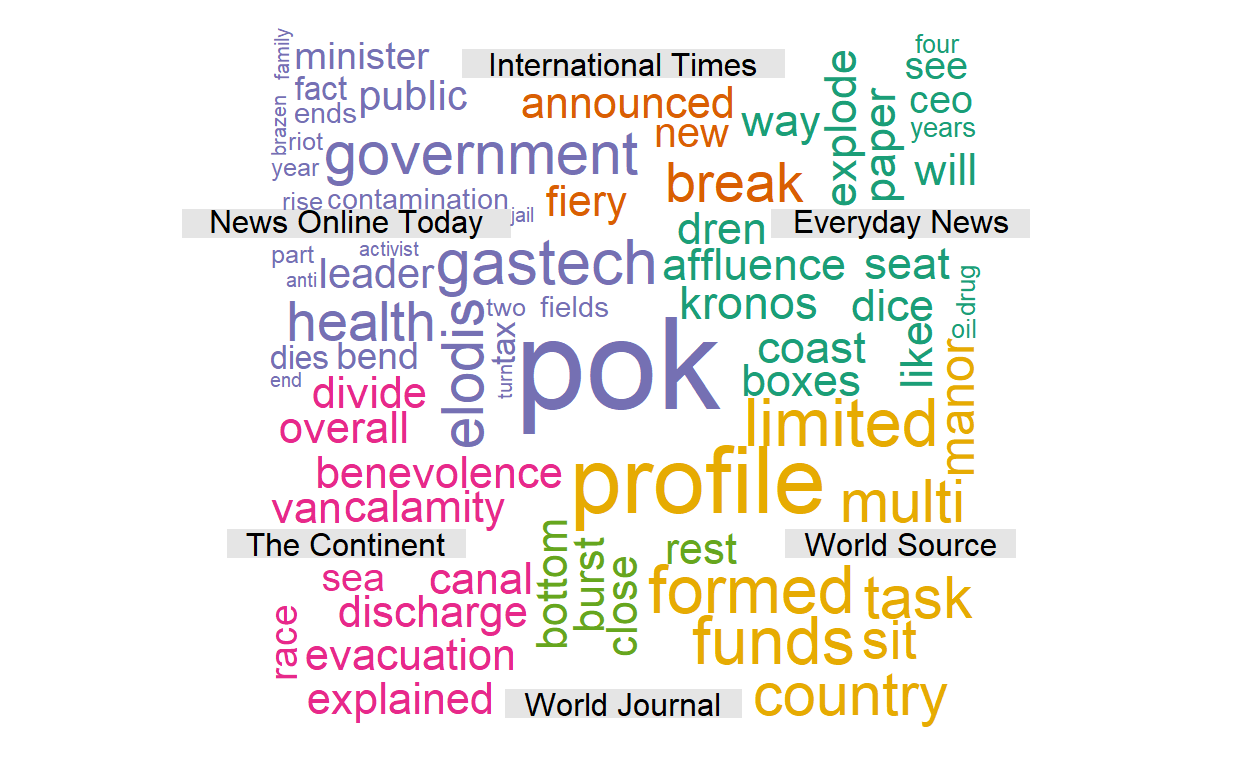
\includegraphics{img/image03.png}

Fig. x above shows the comparison cloud between six newsgroups based on
the words taken from the published news articles' titles. Our
application will have the option for choosing between viewing keywords
from ``Content of Articles'' or ``Titles of Articles''. Moreover, users
can choose the newsgroups they would have to like to compare from a
dropdown list of all the newsgroups available.

The packages used to build this visualisation are \textbf{tidytext},
\textbf{tm} and \textbf{wordcloud}. \textbf{Tidytext} is used to convert
text into a format that is visualisable with the use of `unnext\_tokens'
function. \textbf{tm} has built in functions such as `removeStopwords'
to help in the removal of unimportant words. Lastly, the comparison
cloud will be developed using the \textbf{wordcloud} package.

\textbf{Textnet and Text Plot}

Textnet is used for clustering of newsgroups. To represent the data in
cluster format, the data has to be converted to two columns. The first
column would be the set of words found in news articles and the second
is the name of newsgroups themselves. That way, a network can be created
where newsgroups are connected by their use of the same words, as shown
in Fig. X. The thickness of the edge connecting any two nodes represents
how similar the two nodes are.

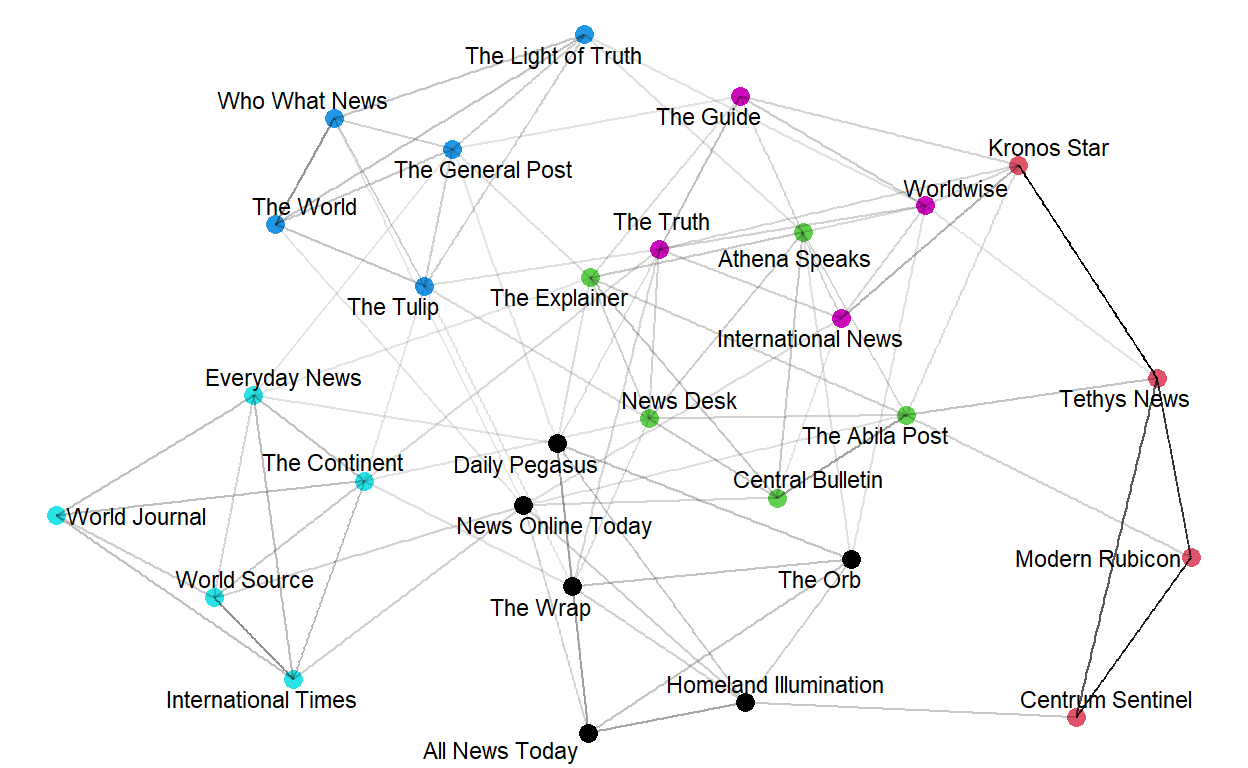
\includegraphics{img/image02.png}

\textless\textless\textless\textless\textless\textless\textless{} HEAD
The node color corresponds to the text communities, with the same color
indicating a strong relationship between its components. In this way,
clusters are formed to segment the newsgroups with similar
characteristics in terms of the types of words used in the news
articles. =======

The node color corresponds to the text communities, with the same colour
indicating a strong relationship between its components. In this way,
clusters are formed to segment the newsgroups with similar
characteristics in terms of the types of words used in the news
articles.
\textgreater\textgreater\textgreater\textgreater\textgreater\textgreater\textgreater{}
55128c1e2b8505f7ba492d07e81bd19206ab1ed8

To delve into the cluster segments of different newsgroup, we visualize
each segmentation as follows:

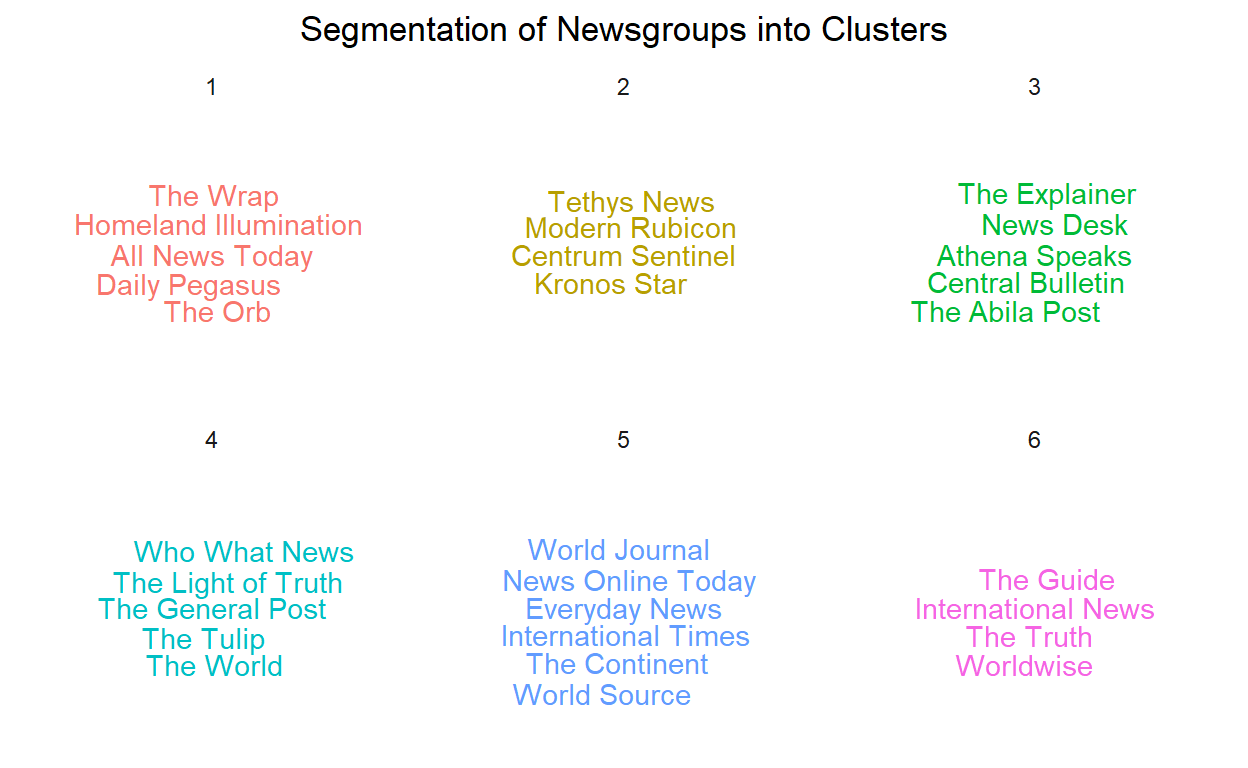
\includegraphics{img/image04.png}

Upon visualizing the components in each cluster, text plot
visualizations are conducted to pull out the word co-occurrences between
word-pairs, so as to determine the context and content of each clusters.

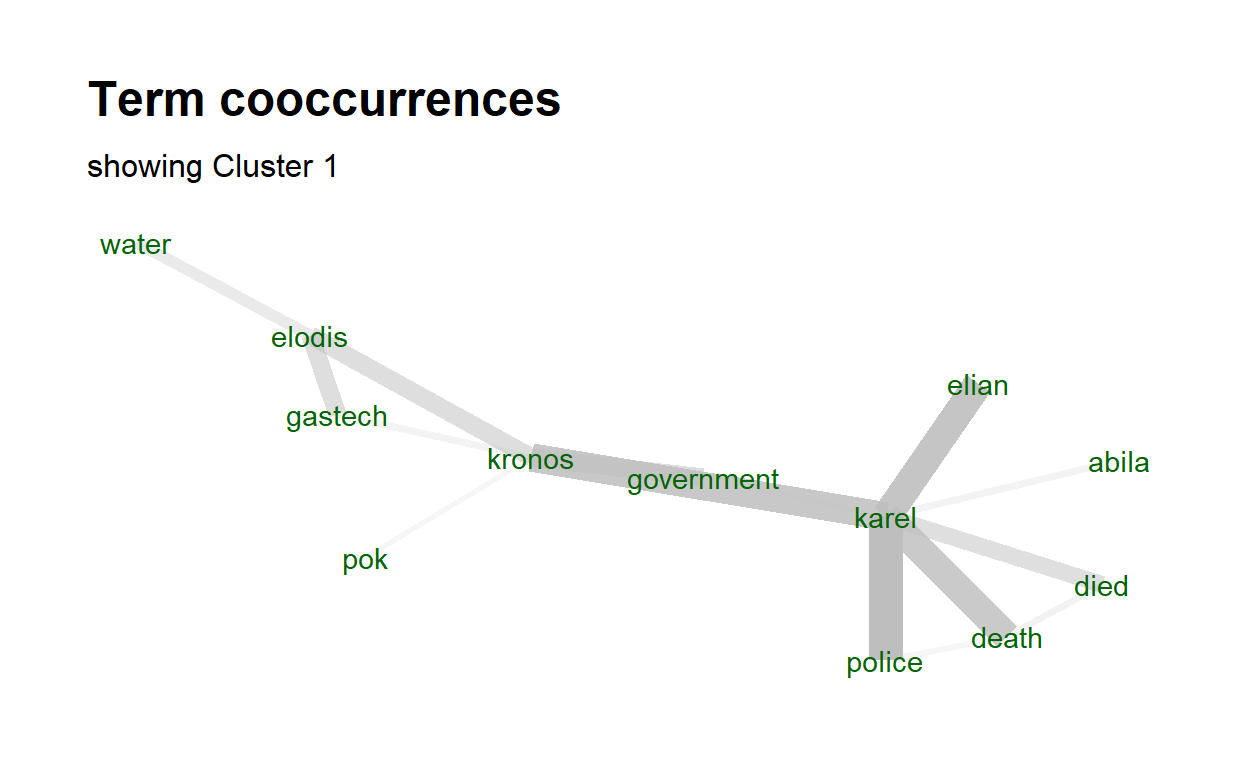
\includegraphics{img/image05.png}

The main R packages used are \textbf{textnet}, \textbf{ggwordcloud},
\textbf{tidytext}, \textbf{udpipe} and \textbf{textplot}.
\textbf{Textnet} is currently the only R package available to implement
text network techniques in R. To display the word cloud by cluster,
\textbf{ggwordcloud} was utilised. \textbf{Tidytext} helps to convert
text into a format that is visualisable with the use of `unnest\_tokens'
function. The \textbf{udpipe} package provides language-agnostic
tokenisation, tagging, lemmatisation and dependency parsing of raw text,
which is an essential part in natural language processing (NLP). Lastly,
to plot data as a text plot, we will be needing the \textbf{textplot}
package.

\textbf{Correlation Graphs} Correlation graphs are plotted to determine
the correlation between different newsgroups. From this, we are able to
determine which newsgroups might be highly related in terms of their
reports of certain events over the years. The correlation values are
obtained using the widely used Pearson method.

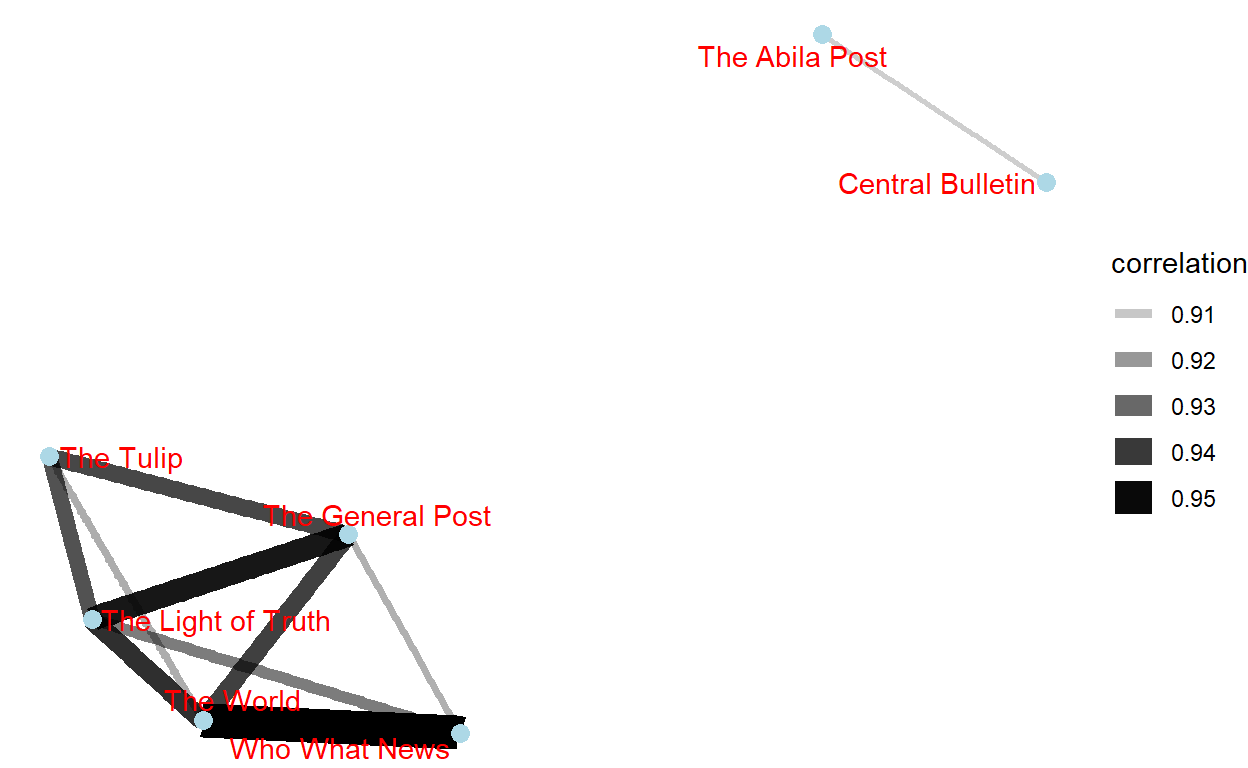
\includegraphics{img/image06.png}

The R packages used are \textbf{widyr} and \textbf{ggraph}.
\textbf{Widyr} is able to cast a tidy dataset into a wide matrix,
performs an operation such as computing the correlation on it, and then
re-tidies the result. `pairwise\_cor' function is found in this package.
\textbf{ggraph} is then used to plot the relationship between different
newsgroups based on their correlation values.

\textless\textless\textless\textless\textless\textless\textless{} HEAD
\textbf{TF-IDF} As mentioned in the \textbf{Review \& Critics of Past
Works} section, word cloud alone might not be very useful to visualize a
collection of `microblog' messages due to its consistency issue. As
such, TF-IDF approach is more helpful when trying to pick out specific
key events/topics of relevance. ======= \textbf{Term Frequency-Inverse
Document Frequency (TF-IDF)}
\textgreater\textgreater\textgreater\textgreater\textgreater\textgreater\textgreater{}
55128c1e2b8505f7ba492d07e81bd19206ab1ed8

As mentioned in the \textbf{Review \& Critics of Past Works} section,
word cloud alone might not be very useful to visualise a collection of
microblog message due to its consistency issue. As such, TF-IDF approach
is more helpful when trying to pick out specific key events/topics of
relevance. This approach aims to measure the importance of a word is to
a document in a collection/corpus of documents, by including the inverse
document frequency (IDF) to balance the term frequency (TF) used in
wordclouds. Hence, we will view each hour of tweets as a document and
all 5 hours of the dataset as the corpus, to determine the key events
that dominate each hour. With that, TF-IDF can be a powerful heuristic
to sieve out the most important events occurring during each period from
the chatter spread throughout the dataset.

We plotted out both unigrams and bigrams to look at both the singular
word and word-pairs respectively.

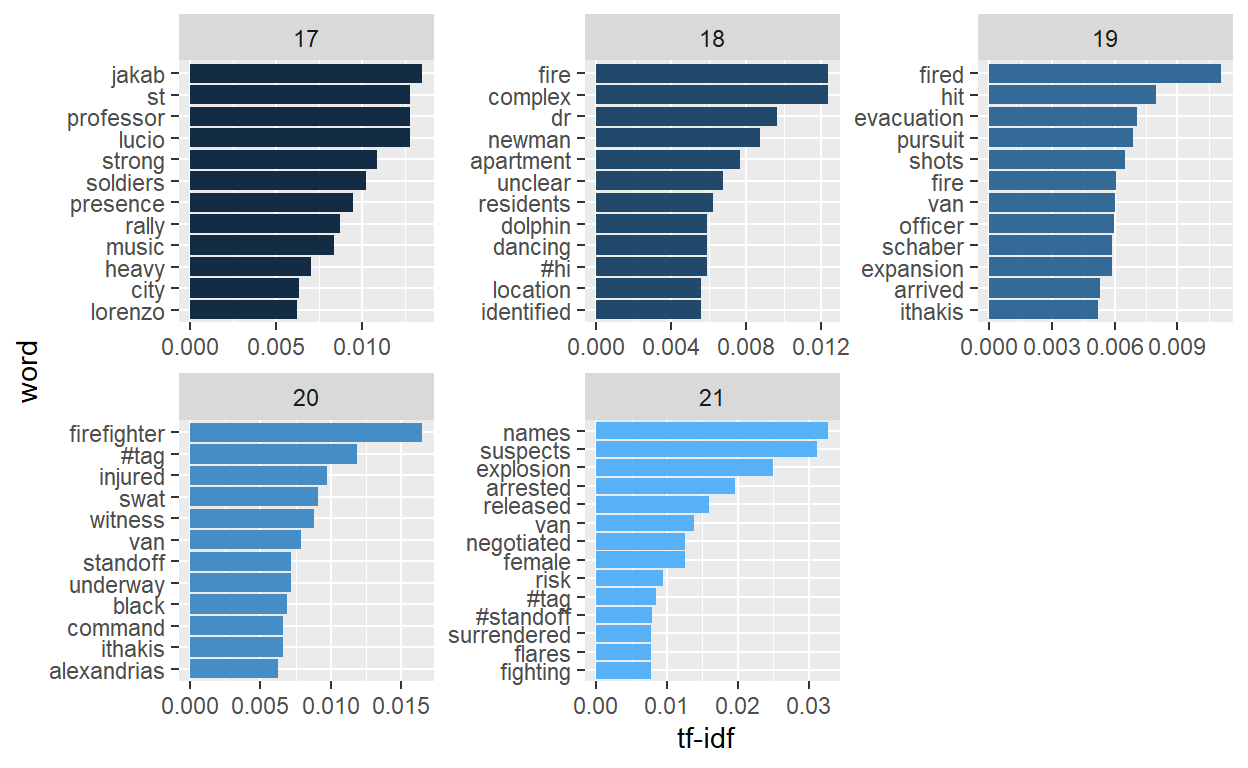
\includegraphics{img/image07.png}

The relevant R package used is \textbf{tidytext}, where the
`bind\_tf\_idf' function helps to compute and bind the term frequency,
inverse document frequency and td-idf of a tidy text dataset to the
dataset.

\hypertarget{network-graphs-1}{%
\subsubsection{Network Graphs}\label{network-graphs-1}}

Network graphs are informative visualisations to mainly show the
relationship between different entities. In this study, network graphs
are created to visualise the different official and unofficial
relationships of GASTech employees and the overall distribution flow of
emails.

\textbf{Email Flow}

The email distribution flow from one person to another is visualised in
terms of a network graph. The thickness of the edge implies the number
of email passed between two nodes. The nodes are grouped by the
employees' \textbf{Current Employment Type}, and users also have the
option to view select the email distribution flow on a daily basis or on
a weekly basis.

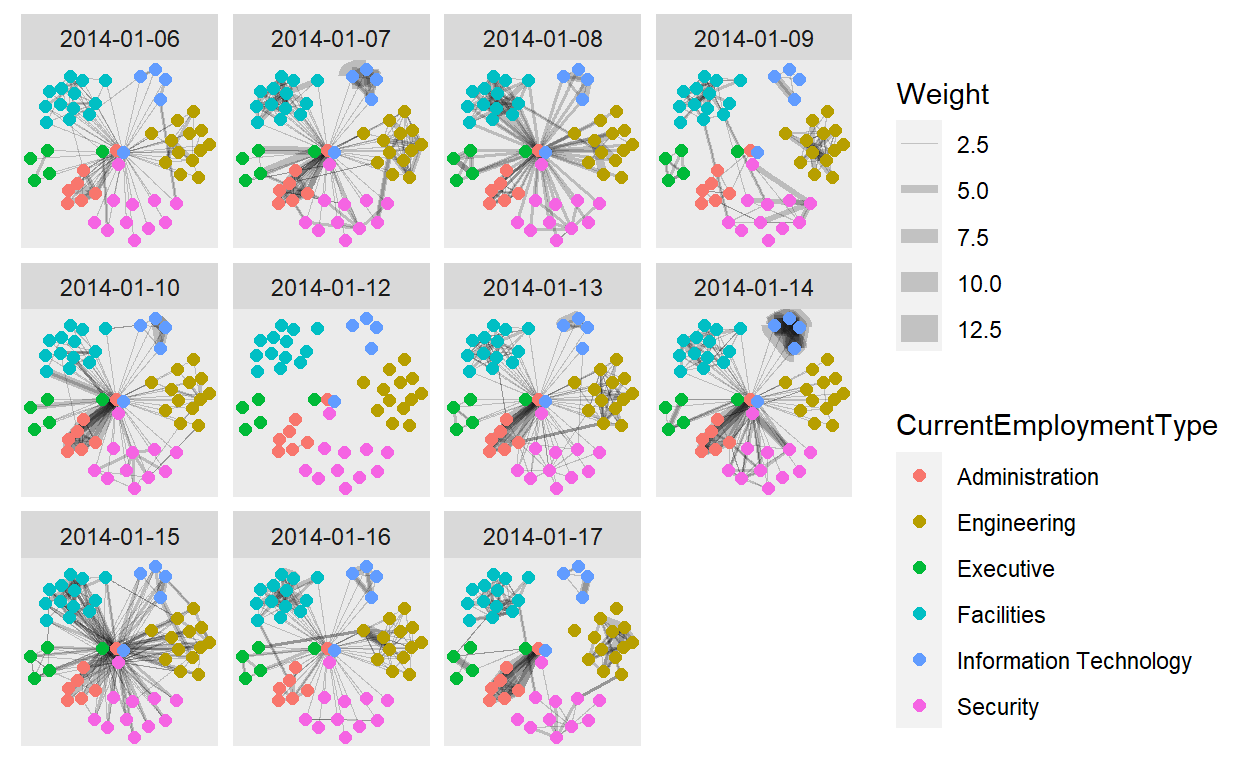
\includegraphics{img/image09.png}

\textbf{Relationships among GASTech Employees}

The email relationships of the employees are split into work-related and
non-work related, in attempt to identify potential suspicious activities
that might be transpiring between different employees. There are four
different views of the network graphs, with the nodes sorted by
``Citizenship'', ``Current Employment Type'', ``Gender'' and ``Current
Employment Title''.

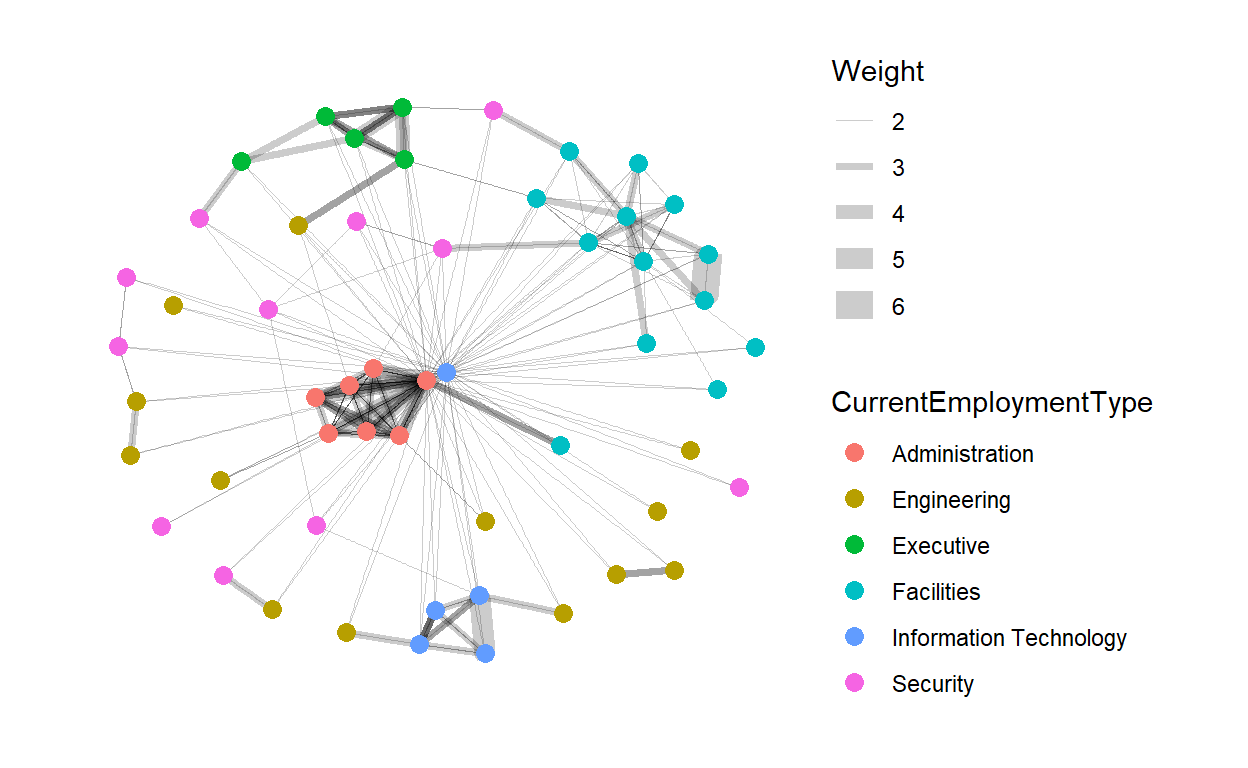
\includegraphics{img/image10.png}

The main R packages needed to create network graphs are
\textbf{tidygraph} and \textbf{ggraph}. Under \textbf{tidygraph}, the
`tbl\_graph' function is used to convert data to an object to display
network belons to this package. \textbf{ggraph} is used to plot the
network object.

\hypertarget{bar-charts}{%
\subsubsection{Bar Charts}\label{bar-charts}}

Separate bar charts are plotted to look into the frequency of the
microblog and call center reports coming in over a fixed time period of
between 1700H to 2200H. Through that, we aim to discover the risk levels
indicated by these data to draw out a basic timeline of major events
that occurred during that evening.

A data table is also linked to the bar chart to show the exact messages
that are received tagged to both time and location.

\textbf{plotly} package is used in this visualisation to be able to
create interactive web-based graphs.

\hypertarget{geospatial-mapping}{%
\subsubsection{Geospatial Mapping}\label{geospatial-mapping}}

Interactive geospatial mapping visualisation is performed so as to track
the locations where those microblogs tweets and call center reports
originate from. The interactive view mode allow layers to be removed or
added, as well as show the exact messages by clicking on the points.

The R package used is \textbf{tmap} to generate thematic maps with high
flexibility and interactivity,

\hypertarget{application-insights}{%
\section{Application Insights}\label{application-insights}}

From our Shiny application, different insights can be drawn to learn
more about the Kronos Incident.

\hypertarget{content-of-newsgroups}{%
\subsection{Content of Newsgroups}\label{content-of-newsgroups}}

Looking into Fig. X, we can observe that ``News Online Today'' is the
newsgroup that mostly talked about the situation in Kronos, with a
majority of articles speaking about POK but little was spoken about the
contamination and health of the Kronos villagers. Hence, this implies
that ``News Online Today'' seems to be targeting the POK group the most.

On the other hand, ``The Continent'' has been reporting on the calamity,
evacuation and discharge, with little spoken about GASTech or POK.
``Everyday News'' reports more on the crashes and explosions occurring
in Kronos.

The remaining three newsgroups appear to be international news outlets
and their keywords vary diversely, with none specifically mentioning
about the situation in Kronos.

\hypertarget{context-of-clusters}{%
\subsection{Context of Clusters}\label{context-of-clusters}}

Clustering separated all of the newsgroups into six different clusters
with the following characteristics:

\begin{itemize}
\item
  Cluster 1 - Relationship between police, government and Elian Karel
\item
  Cluster 2 - POK in general and mentions of GASTech employees
\item
  Cluster 3 - Relationship between police, government and POK
\item
  Cluster 4 - CEO of GASTech company and company's investment plans
\item
  Cluster 5 - Nature of GASTech company as well as relationship between
  govenment and POK
\item
  Cluster 6 - Tension between police and POK + Health situation in
  Kronos
\end{itemize}

\hypertarget{email-flow-and-distribution}{%
\subsection{Email Flow and
Distribution}\label{email-flow-and-distribution}}

Based on the segregration between work related and non-work related
emails, we are able to derive the following insights

\hypertarget{work-related-emails}{%
\subsubsection{Work Related Emails}\label{work-related-emails}}

\begin{itemize}
\tightlist
\item
  Heavy weight assigned to Information Technology, eliminating any
  suspicious activity occurring in this department
\item
  Employees in Engineering department seem to have more communication
  among themselves than the other departments
\item
  One particular IT employee who seems to be communicating with the
  Security and Administration department but not with their own
  department, which raises suspicion
\end{itemize}

\hypertarget{non-work-related-emails}{%
\subsubsection{Non-work Related Emails}\label{non-work-related-emails}}

\begin{itemize}
\tightlist
\item
  Executive Department has more non-work related emails than
  work-related emails
\item
  One IT employee seems to be the most common receiver and sender of
  non-work related emails
\item
  Heavy transmission of unofficial emails among Administration
  Department
\end{itemize}

\hypertarget{microblog-tweets-analysis}{%
\subsection{Microblog Tweets Analysis}\label{microblog-tweets-analysis}}

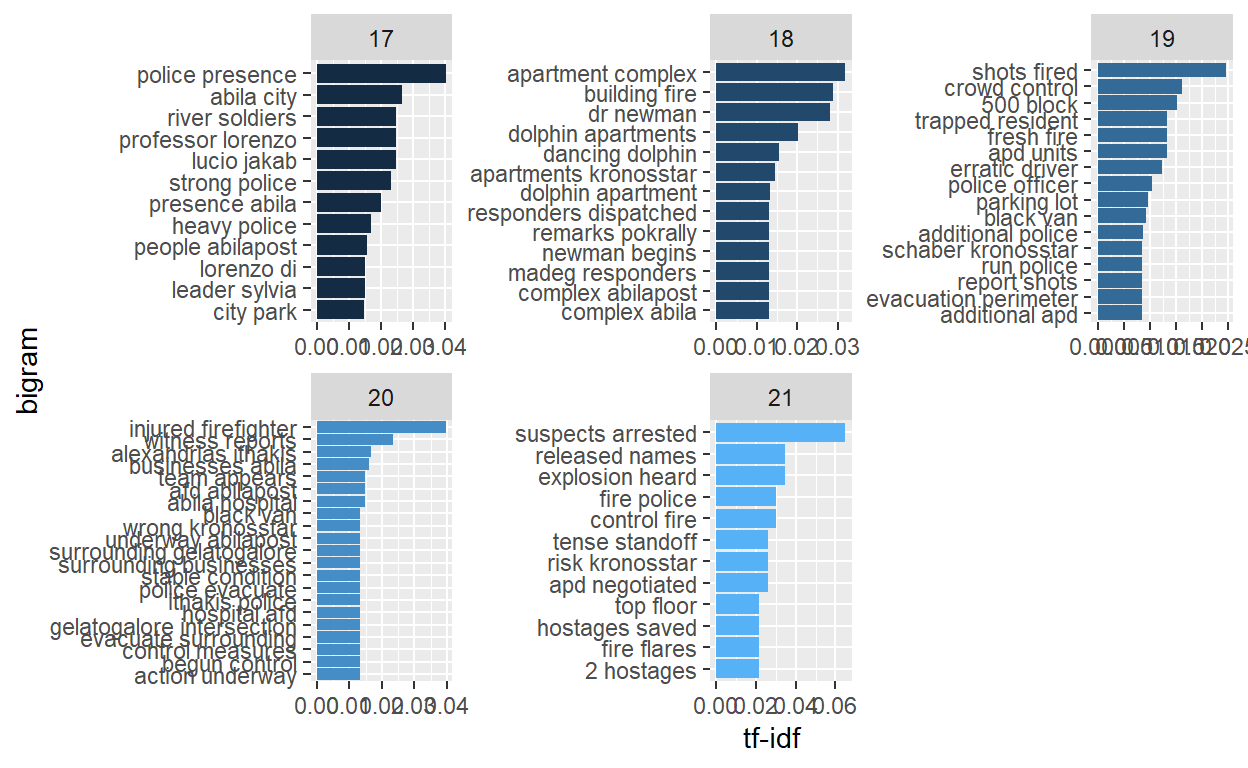
\includegraphics{img/image08.png}

From this bigram plotted, we are able to extract certain important
information as follows:

\begin{itemize}
\tightlist
\item
  1800H+: The fire was likely related to a building, the apartment
  complex of Dancing Dolphon
\item
  1900H+: Shots were fired, with a trapped resident and black van being
  other points of interest.
\item
  2000H+: A firefighter was injured. A phrase ``alexandrias ithakis''
  appears (this is the cross-street where the standoff happened).
  Several businesses appear to be affected as well.
\item
  2100H+: Besides the arrests already spotted in the wordcloud, an
  alarming event of explosions heard also appears.
\end{itemize}

\hypertarget{risk-levels-from-call-center-reports}{%
\subsection{Risk Levels From Call Center
Reports}\label{risk-levels-from-call-center-reports}}

The basic timeline of major event identified over the course of the
evening with its respective risk ratings (on a scale of 1-5, 5 being
highest) are as follows:

\begin{enumerate}
\def\labelenumi{\arabic{enumi}.}
\item
  The first big event was a fire detected at about 1830H (exact time:
  1842H). An ambulance and fire truck was dispatched to the fire. Crowd
  control was also requested. The risk appears to have elevated, but
  appeared under control (risk level 3).
\item
  The next big event happened from 1915H: what appeared as a vehicle
  accident (exact time: 1919H) turned out to be a rogue black van
  running amok in the crowd. It was pursued by police units. Risk level
  would have gone up to 4, due to the uncontrollable nature of the van.
\item
  From 1930H, at least one officer was down because of the event (exact
  time: 1941H). A dire emergency was called, and additional support was
  requested. Risk level would have been at 5 (given that the situation
  was termed ``dire'').
\item
  Nearing the end after the black van and fire incident seemed to have
  died down, from 2045H there were several reports of crime scene
  investigations, with continued suspicious reports. Risk level would be
  at 3 (moderate).
\end{enumerate}

\hypertarget{map-of-key-messages-with-geolocation}{%
\subsection{Map of Key Messages with
Geolocation}\label{map-of-key-messages-with-geolocation}}

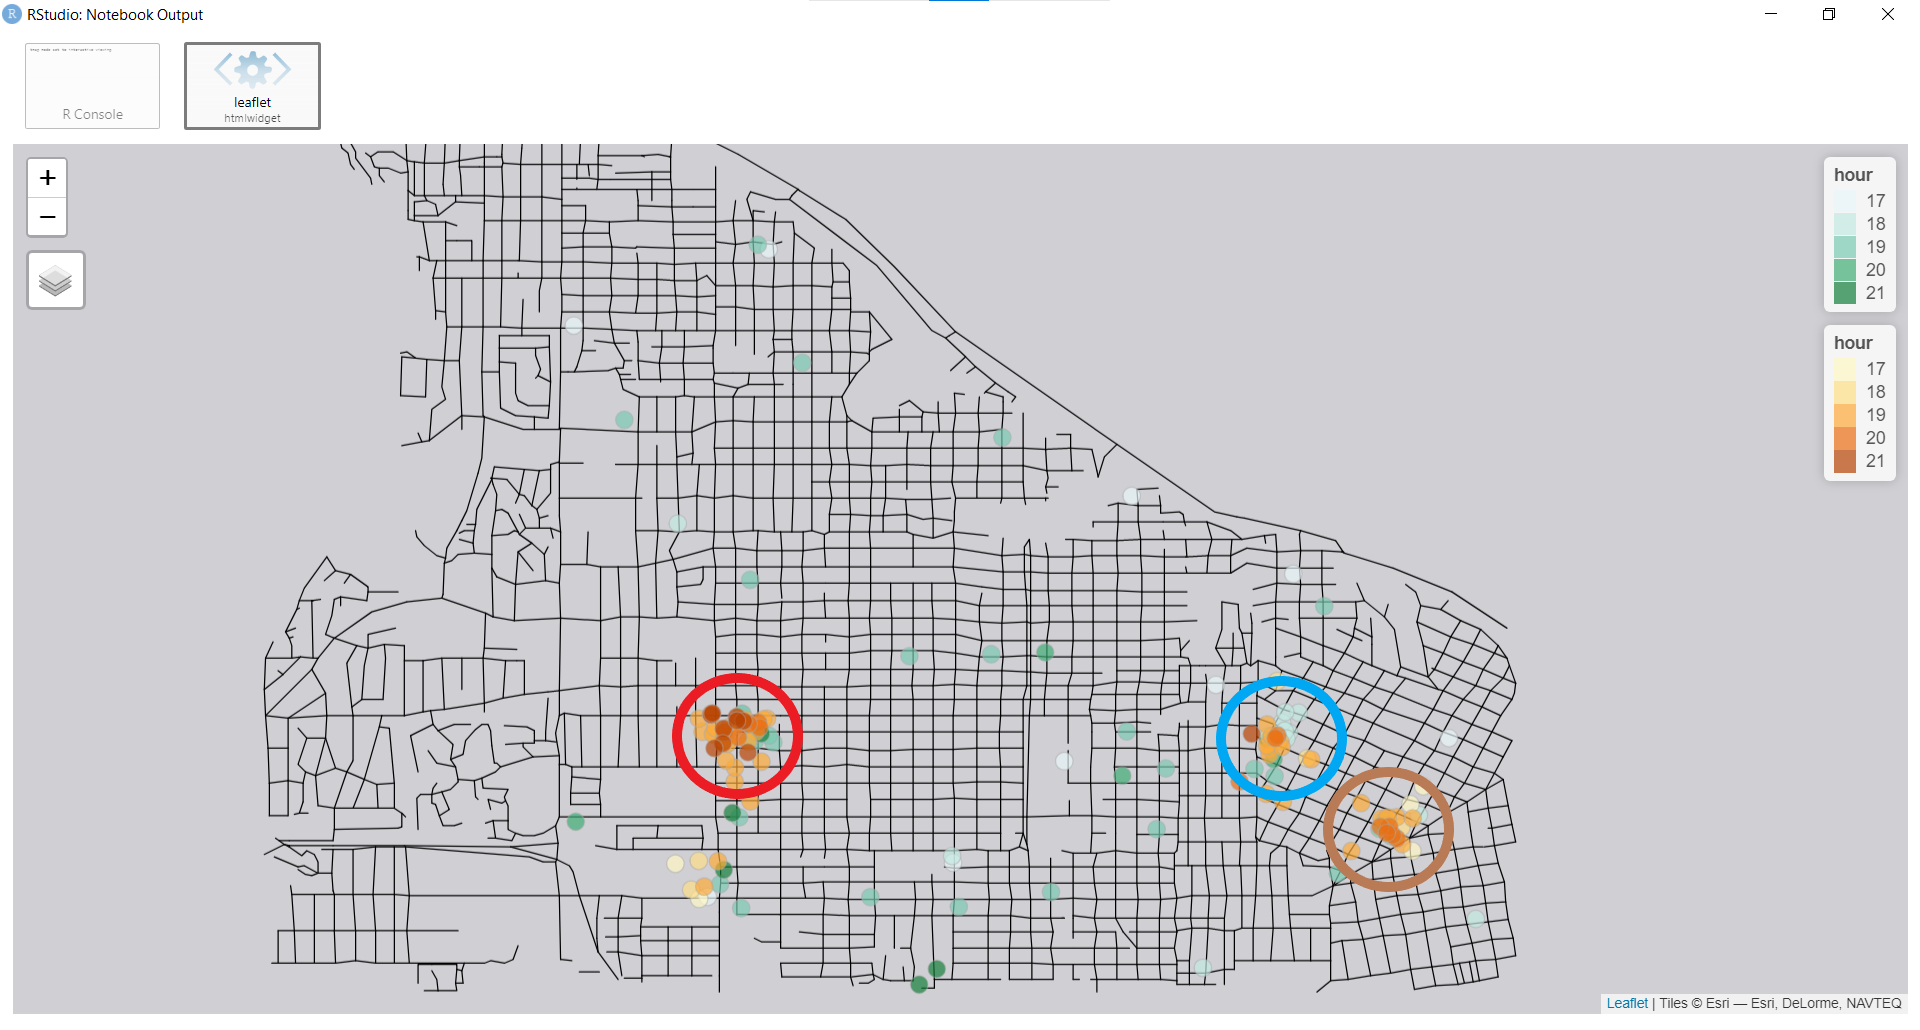
\includegraphics{img/image11.png}

From Fig. X, we are able observe that there are three locations with
high density of message origination, suggesting that major events are
occurring around those location clusters,

The red cluster appears to be the place with highest risk and potential
consequences, due to the high number of negative tweets and several
serious call center reports spread over time. Both types of messages
mention the standoff and police casualties.

The blue cluster also has many call center reports, but lesser negative
tweets. Closer inspection by clicking on the points show that these
tweets are mainly about the fire which appeared to have been under
control, and the call center reports are mostly about dispatch requests.

The brown cluster seems to be about the explosion that occurred late.
Closer inspection shows that many of such messages are sent by a spam
account footfingers.

\hypertarget{conclusion-and-future-work}{%
\section{Conclusion and Future Work}\label{conclusion-and-future-work}}

In conclusion, this study attempts to draw out insights related to the
disappearance of the GASTech employees from a collection of artifacts
and emails related to the GASTech company. The analysis in our web
application is scoped to investigate how events unfolded on the day of
incident and prove the reputation of GASTech since its establishment.

Further developments to the application can be implemented such that
users can upload their own datasets, like text corpus into the
application to conduct text and visual analysis on new datasets.

\hypertarget{references}{%
\section{References}\label{references}}
\setlength{\parindent}{0in}

\end{document}
